\documentclass[12pt]{article}
\usepackage[utf8]{inputenc}
\usepackage[T1]{fontenc}
\usepackage[brazil]{babel}
\usepackage{geometry}
\geometry{a4paper, top=2.5cm, bottom=2.5cm, left=2.5cm, right=2.5cm}
\usepackage{graphicx}
\usepackage{booktabs}
\usepackage{amsmath}
\usepackage{hyperref}

\title{\textbf{Implementação e Avaliação Experimental das Organizações MIPS32 Monociclo (O1) e Pipeline de 5 Estágios (O2)}}
\author{Alonso Fernandes Cavalcante\\
Departamento de Ciência da Computação -- Universidade Federal de Roraima (DCC/UFRR)\\
Boa Vista -- RR -- Brasil}
\date{2026}

\begin{document}
\maketitle

\begin{abstract}
Este trabalho apresenta o projeto em VHDL-2008, a verificação funcional e a avaliação experimental de desempenho de duas organizações microarquiteturais para um subconjunto de 10 instruções do MIPS32: Monociclo (\textbf{O1}) e Pipeline escalar de 5 estágios (\textbf{O2}) com Unidade de Detecção de Conflitos (RAW, estrutural e de controle) e congelamento arquitetural. A corretude funcional é validada contra o simulador MARS 4.5 por meio de um testbench único (\texttt{tb\_cpu.vhd}). Com base na regra única de caminho crítico e nos atrasos da Figura 4.27 de Patterson e Hennessy (Seção 4.5, p. 273), obtêm-se períodos de clock de $0{,}80\text{ ns}$ em \textbf{O1} e $0{,}20\text{ ns}$ em \textbf{O2} (razão de clock de $4{,}00\times$). Os resultados sobre o traço \texttt{T0} e a Série \texttt{S} (\texttt{S5} a \texttt{S200}) demonstram que o speedup medido evolui de $2{,}40\times$ (\texttt{S5}) até $3{,}92\times$ (\texttt{S200}), quantificando o efeito do desequilíbrio entre estágios e dos 4 ciclos de enchimento e esvaziamento do pipeline.
\end{abstract}

\section{Introdução}
A técnica de \textit{pipelining} divide a execução das instruções em estágios sequenciais isolados por registradores, permitindo sobrepor múltiplas instruções e reduzir o período do relógio ao atraso do estágio mais lento \cite{patterson2017}. Este relatório descreve a implementação e avaliação comparativa das organizações \textbf{O1 (Monociclo)} e \textbf{O2 (Pipeline de 5 estágios)} para o subconjunto MIPS32 composto por \texttt{add}, \texttt{sub}, \texttt{and}, \texttt{or}, \texttt{slt}, \texttt{addi}, \texttt{lw}, \texttt{sw}, \texttt{beq} e \texttt{break}.

\section{Arquitetura das Organizações O1 e O2}
\subsection{Escolha da Linha de Base O1 e Componentes Compartilhados}
Adotou-se a organização \textbf{Monociclo} como linha de base (\textbf{O1}) em vez de uma organização Multiciclo. Uma organização Multiciclo introduziria uma máquina de estados com $\text{CPI} > 1$ variável por classe de instrução, mesclando variações de CPI e de período de clock. O Monociclo mantém $\text{CPI}_{\text{útil}} = 1{,}0$ constante, servindo como referência de ciclos e tempo de execução para cálculo de \textit{speedup}, enquanto o simulador \textbf{MARS 4.5} atua como oráculo funcional. Ambas as organizações compartilham os mesmos módulos em \texttt{comum/} (ULA, controle da ULA, extensor de sinal, banco de 32 registradores e memórias de instruções e dados de 1024 palavras = 4 KB com endereçamento modular \textit{wrap-around}).

\subsection{Pipeline O2, Registradores Entre Estágios e Hazards}
A organização \textbf{O2} subdivide o caminho de dados nos estágios \textbf{IF}, \textbf{ID}, \textbf{EX}, \textbf{MEM} e \textbf{WB}, separados por quatro registradores que totalizam \textbf{426 bits}: \texttt{IF/ID} (65 bits), \texttt{ID/EX} (149 bits), \texttt{EX/MEM} (107 bits) e \texttt{MEM/WB} (105 bits). O banco de registradores realiza a escrita do estágio \texttt{WB} na borda de descida (\textit{meio ciclo}) e a leitura combinacional de \texttt{ID} na 2ª metade do ciclo, tornando distâncias $\ge 3$ livres de conflitos RAW.

A Unidade de Detecção de Hazards monitora: (i) \textbf{RAW (tipo \texttt{01})} no estágio \texttt{ID} contra instruções produtoras válidas em \texttt{EX} (distância 1) ou \texttt{MEM} (distância 2) com destino diferente de \texttt{\$zero}; (ii) \textbf{Estrutural (tipo \texttt{10})} quando \texttt{MEM\_UNIFICADA = true} e \texttt{IF} e \texttt{MEM} acessam a memória simultaneamente; e (iii) \textbf{Controle (tipo \texttt{11})} no estágio \texttt{EX} quando um desvio \texttt{beq} é tomado (\texttt{ex\_take\_branch = '1'}) com instruções sequenciais já buscadas em \texttt{ID} ou \texttt{IF}. Quando \texttt{beq} não é tomado, as instruções em \texttt{PC+4} e \texttt{PC+8} pertencem ao fluxo correto e não há conflito.

\section{Metodologia Experimental e Ameaças à Validade}
\subsection{Regra Única de Período de Clock e Restrição de Meio Ciclo}
Aplicou-se a mesma regra de temporização a ambas as organizações: \textit{o período de clock mínimo ($T_{\text{clk}}$) é dado pelo maior atraso entre dois elementos de estado consecutivos ($T_{\text{caminho\_max}} + t_{\text{reg}}$), respeitando a restrição de meio ciclo do banco de registradores ($T_{\text{clk}}/2 \ge \max(t_{\text{RegWrite}}, t_{\text{RegRead}})$)}. Pela Figura 4.27 (Seção 4.5, p. 273) de \cite{patterson2017} ($t_{\text{IMEM}} = 200\text{ ps}$, $t_{\text{RegRead}} = 100\text{ ps}$, $t_{\text{ULA}} = 200\text{ ps}$, $t_{\text{DMEM}} = 200\text{ ps}$, $t_{\text{RegWrite}} = 100\text{ ps}$ e hipótese $t_{\text{reg}} = 0\text{ ps}$):
\begin{equation}
T_{\text{clk, O1}} = 200 + 100 + 200 + 200 + 100 = 800\text{ ps } (0{,}80\text{ ns})
\end{equation}
\begin{equation}
T_{\text{clk, O2}} = \max(200, 100, 200, 200, 100) = 200\text{ ps } (0{,}20\text{ ns})
\end{equation}
Em \textbf{O2}, metade do período vale $T_{\text{clk, O2}}/2 = 100\text{ ps}$, acomodando exatamente a escrita de \texttt{WB} ($100\text{ ps}$) na 1ª metade e a leitura de \texttt{ID} ($100\text{ ps}$) na 2ª metade do ciclo.

\subsection{Ameaças à Validade}
Destacam-se três ameaças à validade: (1) no RTL simulado de \textbf{O1}, o módulo \texttt{banco\_reg} compartilha a escrita na borda de descida com \textbf{O2}; em síntese física real, exigir que o caminho de \texttt{lw} coubesse em meio ciclo dobraria o período de \textbf{O1}, razão pela qual adotou-se a fórmula clássica de fim de ciclo ($0{,}80\text{ ns}$) para análise justa; (2) desprezou-se o overhead físico de registradores ($t_{\text{reg}} = 0\text{ ps}$), conforme a Figura 4.27 do livro-texto; e (3) os traços limpos possuem distância $\ge 3$ e desvios não tomados.

\section{Resultados Experimentais e Análise Crítica}
A Tabela \ref{tab:metricas} sintetiza os resultados obtidos para o traço principal \texttt{T0} e para a Série \texttt{S} (variações de \texttt{T0} com todas as classes da ISA e 0 erros nos 32 registradores). Os traços de conflito abortaram exatamente nos ciclos e endereços esperados: \texttt{TD} (tipo \texttt{01}, \texttt{PC=0x04}, ciclo 3), \texttt{TE} (tipo \texttt{10}, \texttt{PC=0x0C}, ciclo 4) e \texttt{TC} (tipo \texttt{11}, \texttt{PC=0x00}, ciclo 3).

\begin{table}[htb]
\centering
\caption{Métricas de Desempenho Consolidada para T0 e Série S (0 erros)}
\label{tab:metricas}
\small
\begin{tabular}{lccccccccc}
\toprule
\textbf{Traço} & $N$ & \textbf{Ciclos O1} & \textbf{Ciclos O2} & \textbf{CPI O1} & \textbf{CPI O2} & $T_{\text{O1}}$ (ns) & $T_{\text{O2}}$ (ns) & \textbf{Ocup. O2} & \textbf{Speedup} \\
\midrule
\texttt{S5}   & 5   & 6   & 10  & 1,2000 & 2,0000 & 4,80  & 2,00  & 60,00\% & \textbf{2,4000$\times$} \\
\texttt{S10}  & 10  & 11  & 15  & 1,1000 & 1,5000 & 8,80  & 3,00  & 73,33\% & \textbf{2,9333$\times$} \\
\texttt{S20}  & 20  & 21  & 25  & 1,0500 & 1,2500 & 16,80 & 5,00  & 84,00\% & \textbf{3,3600$\times$} \\
\texttt{T0}   & 31  & 32  & 36  & 1,0323 & 1,1613 & 25,60 & 7,20  & 88,89\% & \textbf{3,5556$\times$} \\
\texttt{S50}  & 50  & 51  & 55  & 1,0200 & 1,1000 & 40,80 & 11,00 & 92,73\% & \textbf{3,7091$\times$} \\
\texttt{S100} & 100 & 101 & 105 & 1,0100 & 1,0500 & 80,80 & 21,00 & 96,19\% & \textbf{3,8476$\times$} \\
\texttt{S200} & 200 & 201 & 205 & 1,0050 & 1,0250 & 160,80& 41,00 & 98,05\% & \textbf{3,9220$\times$} \\
\bottomrule
\end{tabular}
\end{table}

\begin{figure}[htb]
\centering
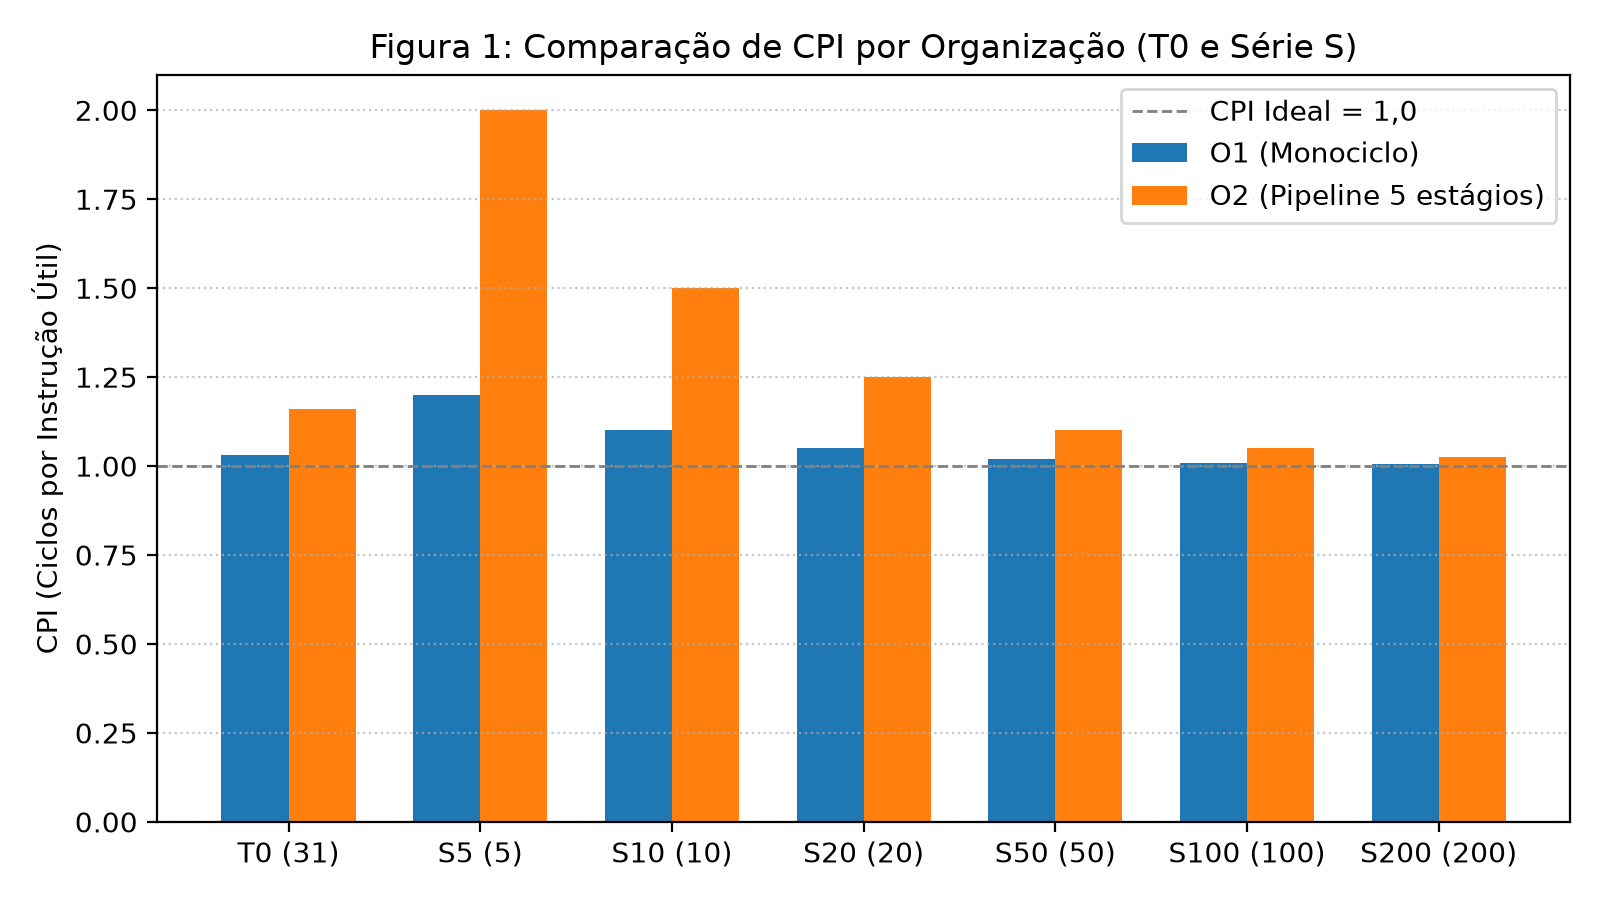
\includegraphics[width=0.78\textwidth]{../graficos/fig1_cpi.png}
\caption{Comparação de CPI por organização para T0 e Série S.}
\end{figure}

\begin{figure}[htb]
\centering
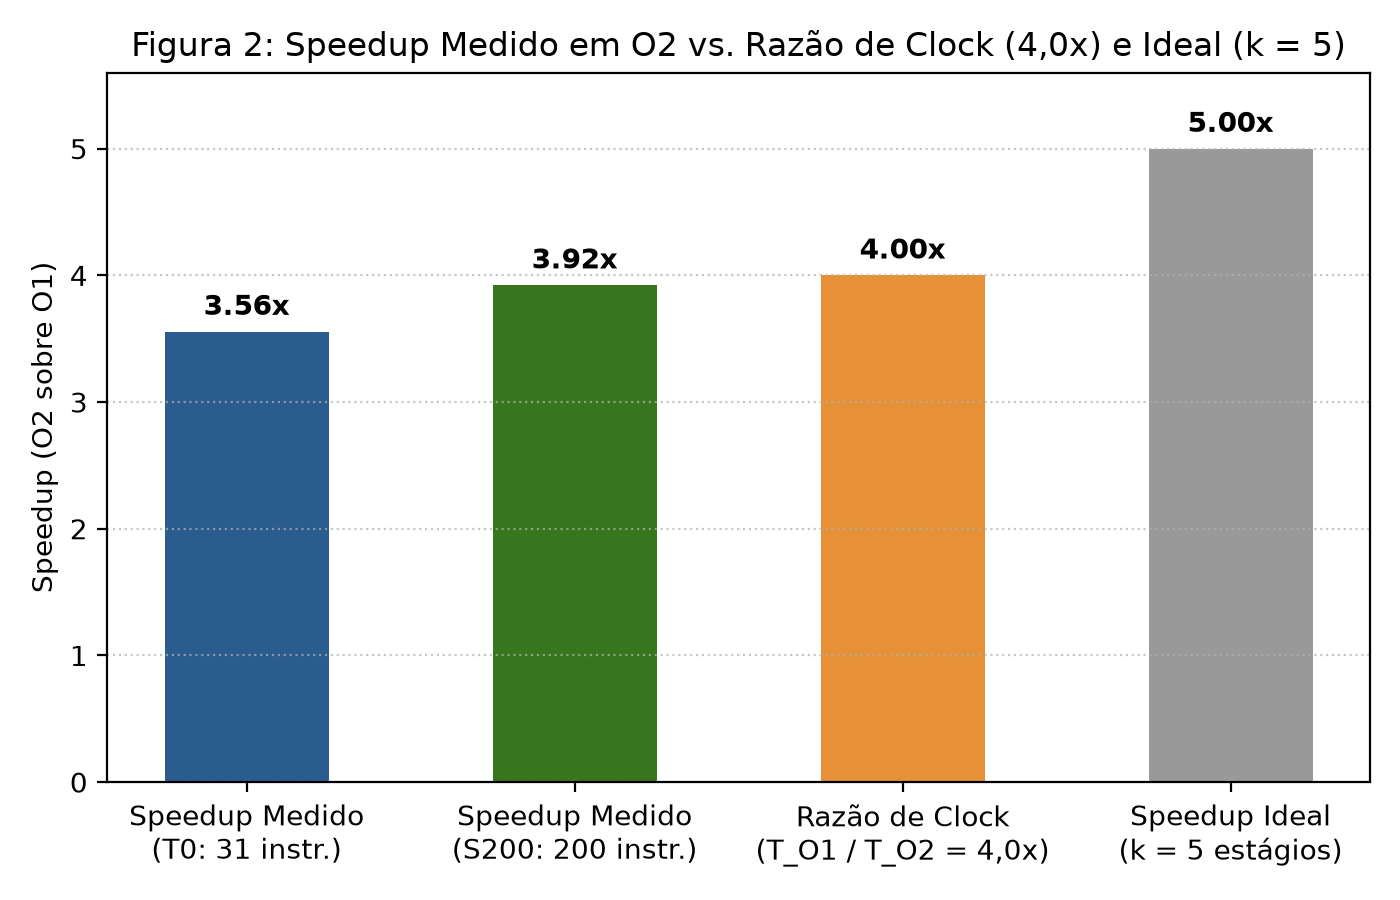
\includegraphics[width=0.72\textwidth]{../graficos/fig2_speedup_ideal.png}
\caption{Speedup medido em T0 e S200 frente à Razão de Clock ($4{,}0\times$) e ao limite ideal ($k=5$).}
\end{figure}

\begin{figure}[htb]
\centering
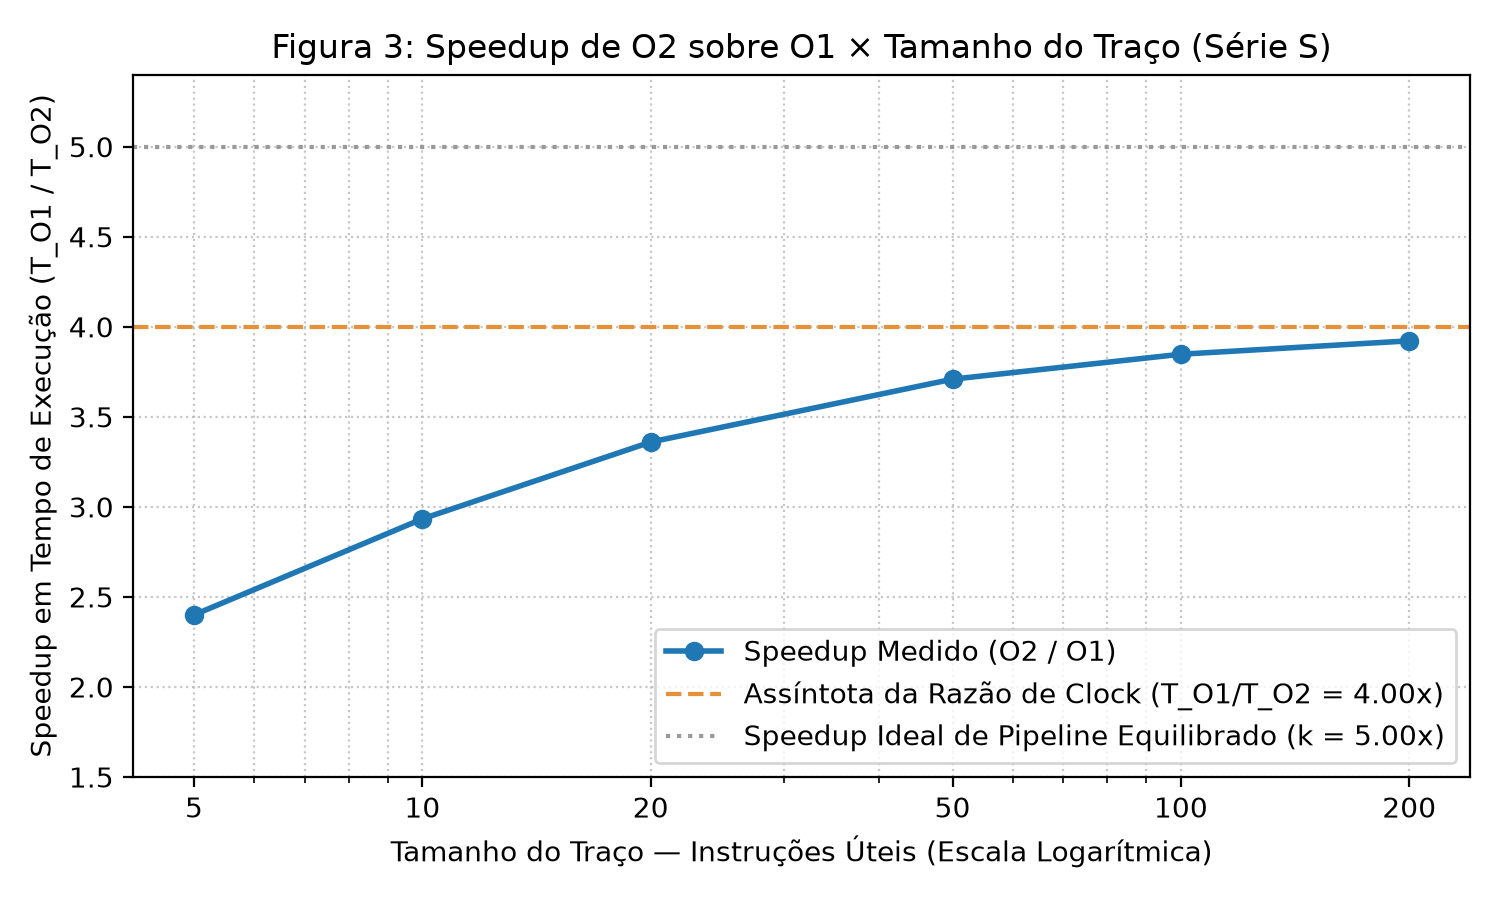
\includegraphics[width=0.78\textwidth]{../graficos/fig3_speedup_serie_s_log.png}
\caption{Curva de convergência do Speedup de O2 sobre O1 na Série S (escala logarítmica).}
\end{figure}

\textbf{Discussão Crítica}: O limite ideal clássico de um pipeline de 5 estágios ($k = 5{,}00\times$) exige que todos os estágios sejam perfeitamente equilibrados ($160\text{ ps}$ cada). Como em \textbf{O2} os estágios \texttt{IF}, \texttt{EX} e \texttt{MEM} duram $200\text{ ps}$ enquanto \texttt{ID} e \texttt{WB} duram $100\text{ ps}$, o desequilíbrio limita a razão assintótica de clock a $T_{\text{clk, O1}}/T_{\text{clk, O2}} = 800/200 = 4{,}00\times$. Além disso, para um traço finito de $N$ instruções úteis, \textbf{O2} exige 4 ciclos adicionais de esvaziamento ($N+5$ ciclos contra $N+1$ em \textbf{O1}), fazendo com que o speedup siga a lei $\text{Speedup}(N) = 4{,}00 \times (N+1)/(N+5)$, partindo de $2{,}40\times$ em \texttt{S5} e atingindo $3{,}922\times$ ($98{,}05\%$ da assíntota de clock) em \texttt{S200}.

\begin{thebibliography}{1}
\bibitem{patterson2017}
PATTERSON, D. A.; HENNESSY, J. L. \textit{Organização e Projeto de Computadores: A Interface Hardware/Software}. 5. ed. Rio de Janeiro: Elsevier, 2017. Seção 4.5, Figura 4.27, p. 273.
\end{thebibliography}

\end{document}
